\section{Motivation}\label{motivation}

\begin{frame}{Why bipedal walking?}

\begin{itemize}
\itemsep1pt\parskip0pt\parsep0pt
\item
  Robots should be able to navigate in environments made for humans:

  \begin{itemize}
  \itemsep1pt\parskip0pt\parsep0pt
  \item
    Little space
  \item
    Obstacles (e.g.~stairs)
  \end{itemize}
\end{itemize}

\(\Rightarrow\) Wheeled base not flexible enough.

\begin{itemize}
\itemsep1pt\parskip0pt\parsep0pt
\item
  \textbf{Problem:} How do you guarantee stability during walking?
\end{itemize}

\end{frame}

\begin{frame}{The Human Gait}

\begin{itemize}
\itemsep1pt\parskip0pt\parsep0pt
\item
  Of primary interest for stability: Number of feet that are in contact
  with ground
\item
  Dual support phase: Shift weight from last support leg to next one
\item
  Single support phase: Move swing leg to next foot position
\end{itemize}

\begin{figure}[b]
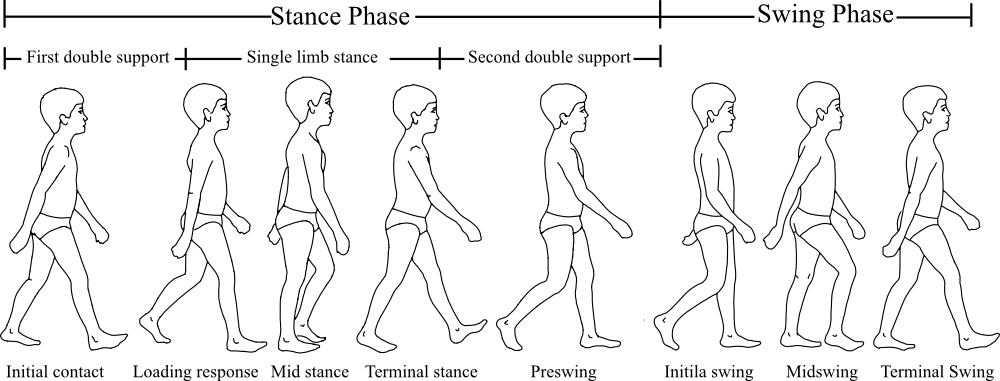
\includegraphics[width=\textwidth,resolution=300]{images/human_gait.png}
\center{
\tiny{Source: Dynamics of Human Gait}
}
\end{figure}

\end{frame}

\begin{frame}{Application to robots?}

\begin{enumerate}
\def\labelenumi{\arabic{enumi}.}
\item
  Adapt recorded human motions to robot:

  \begin{itemize}
  \item
    Kinematic structure and dynamic properties are different: Mapping
    needs to be found.
  \item
    Mapping is computationally expensive (offline), but trajectory looks
    very natural
  \end{itemize}
\item
  Derive stable trajectories from dynamic models of the robot:

  \begin{itemize}
  \item
    Most popular: 3D-Linear Inverted Pendulum Model and ZMP
  \item
    Simplification: Height of the CoM is constant with respect to ground
    (only approximately true for humans see Orendurff et al.
    \cite{orendurff2004effect})
  \item
    Can be computed online, but looks less natural
  \end{itemize}
\end{enumerate}

This work is build on the second approach.

\end{frame}

\begin{frame}{3D Linear Inverted Pendulum Model}

\begin{columns}
\begin{column}{0.55\textwidth}
\begin{itemize}
\item Simplified dynamic description of robot
\item Reduce robot to pendulum with massless rod and point contact
\item \textit{Linear actuator} in rod of pendulum
\item Mass of robot gets reduced to the \textit{CoM} $c = (c_x, c_y)^T$ (the head of the pendulum)
\item To make the dynamics \textit{linear} we constrain the head of the pendulum
to a constant height
\end{itemize}

\end{column}

\begin{column}{0.45\textwidth}
\begin{figure}
  \begin{center}
     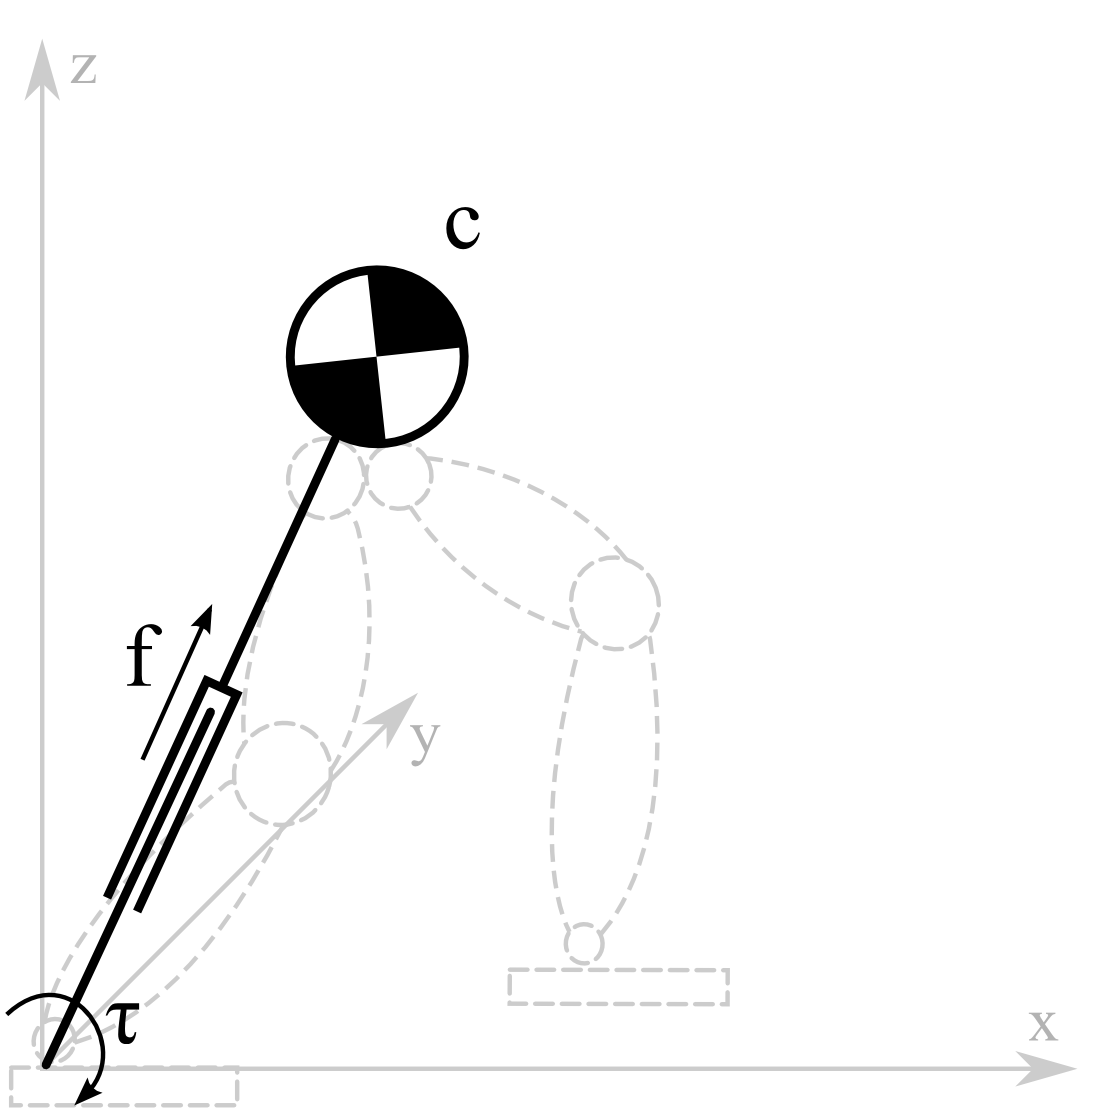
\includegraphics[width=\textwidth]{images/3dlimp.png}
  \end{center}
\end{figure}

\vspace{-1.5em}
Resulting Equation:
\begin{equation*}
\ddot{c}_x = \frac{g}{z_c} c_x
\end{equation*}

\end{column}
\end{columns}

\end{frame}

\begin{frame}{Contact forces}

We can reduce all contact forces acting on the foot to a single force at
the \emph{Center of Pressure} which is computed as:

\begin{columns}
\begin{column}{0.5\textwidth}
\begin{equation*} \label{eq:zmp-definition}
p := \left(\begin{array}{c}
p_x \\ p_y \\ p_z
\end{array}\right)
   = \frac{\sum^N_{i=1}p_i f_{iz}}{\sum^N_{i=1} f_{iz}}
\end{equation*}
\end{column}

\begin{column}{0.5\textwidth}
\begin{figure}[b]
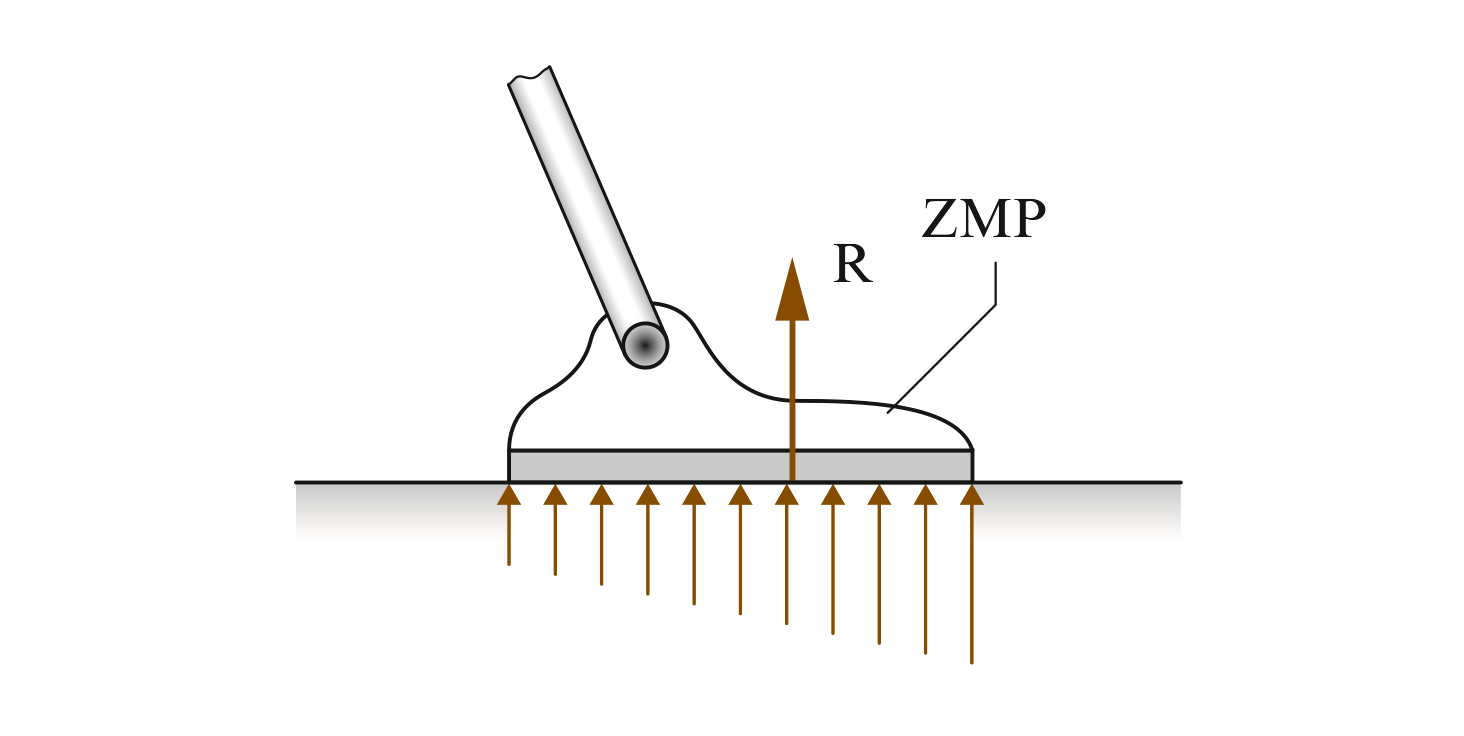
\includegraphics[width=\textwidth,resolution=300]{images/contact_forces.png}
\end{figure}
\end{column}
\end{columns}

\begin{itemize}
\itemsep1pt\parskip0pt\parsep0pt
\item
  If all contact forces are in the same plane: Torque around \(x\) and
  \(y\) axis at this point is zero
\item
  Thus we can call this point the \emph{Zero Moment Point} (ZMP).
\end{itemize}

\end{frame}

\begin{frame}{Why is the ZMP interesting?}

\begin{enumerate}
\def\labelenumi{\arabic{enumi}.}
\item
  Describes the \emph{foot-floor contact dynamics} in case of flat
  ground contact
\item
  Can be used to derive a \emph{condition to ensure dynamically stable
  pose}: If the ZMP is \textbf{strictly inside the support polygon}, the
  foot-floor contact will be preserved.
\end{enumerate}

Use 2. to derive dynamically stable trajectory by constraining ZMP to
support polygones:

\begin{figure}[b]
\includegraphics[width=0.5\textwidth,resolution=300]{images/zmp_steps.png}
\end{figure}

\end{frame}

\begin{frame}{Cart-Table-Model}

\begin{columns}
\begin{column}{0.5\textwidth}
\begin{itemize}
\item Simple model to compute the ZMP
\item Does not require knowledge about contact forces
\item For each dimension: Cart on massless table
\item Cart represents the CoM of the robot
\item Foot of the table corresponds to the support polygon
\end{itemize}

Resulting ZMP:
\begin{equation*} \label{eq:zmp-x}
p_x = c_x - \frac{z_c}{g} \ddot{c_x}
\end{equation*}
\end{column}

\begin{column}{0.5\textwidth}
\begin{figure}
  \begin{center}
     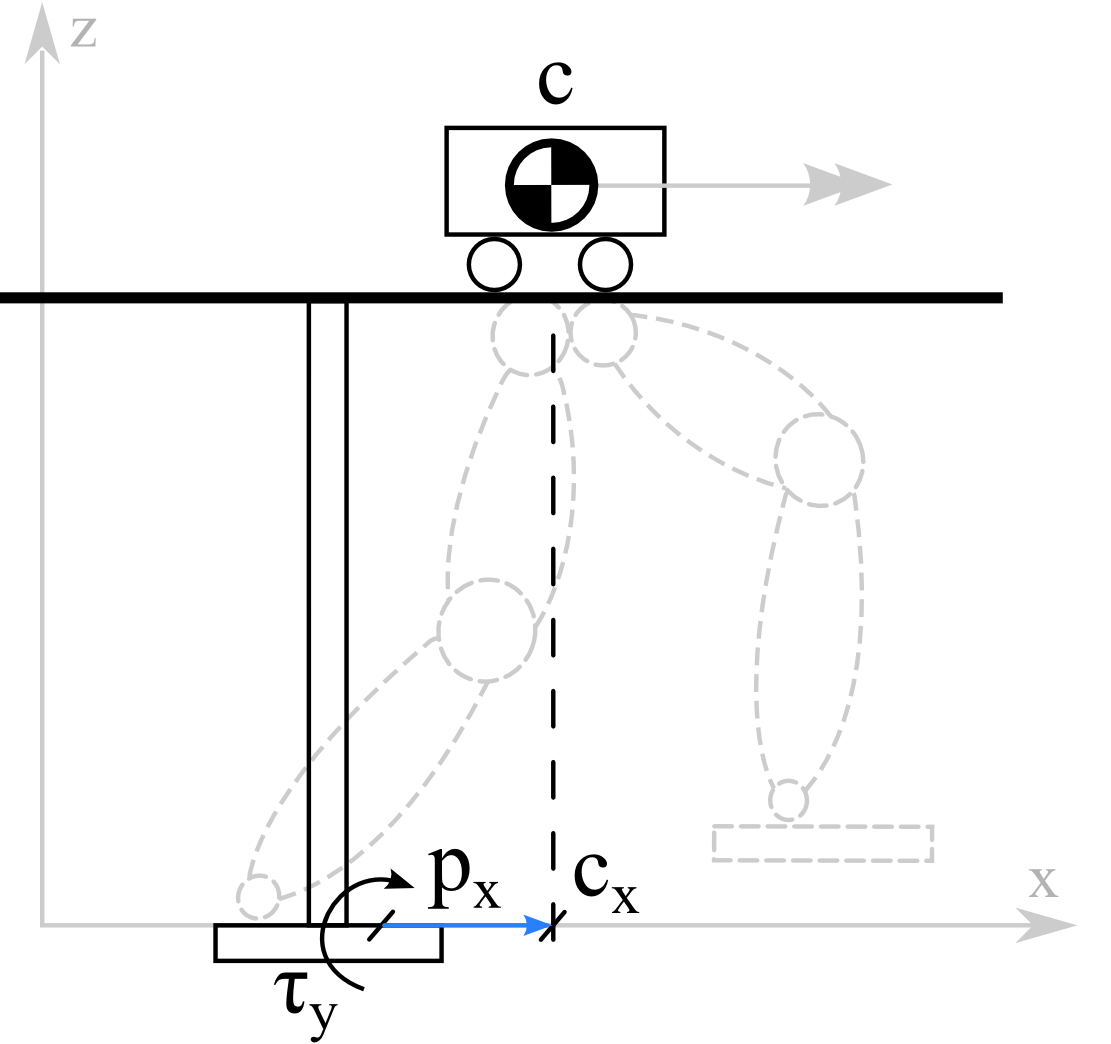
\includegraphics[width=\textwidth]{images/carttable.png}
  \end{center}
\end{figure}
\end{column}
\end{columns}

\end{frame}

\section{Walking Pattern Generation}\label{walking-pattern-generation}

\begin{frame}{Pattern generation as control problem}

\begin{itemize}
\itemsep1pt\parskip0pt\parsep0pt
\item
  \textbf{Idea:} Formulate dynamic walking as a control problem
\item
  \textbf{Goal:} Realize given reference ZMP position
\item
  \textbf{Result:} Array of system states (position, velocity,
  acceleration of the CoM and realized ZMP position)
\item
  \textbf{Implementation}: Uses a Preview Controller (Kajita et al. 2003
  \cite{kajita2003biped}) that utilizes knowledge about the future
  trajectory
\end{itemize}

\begin{figure}
  \begin{center}
     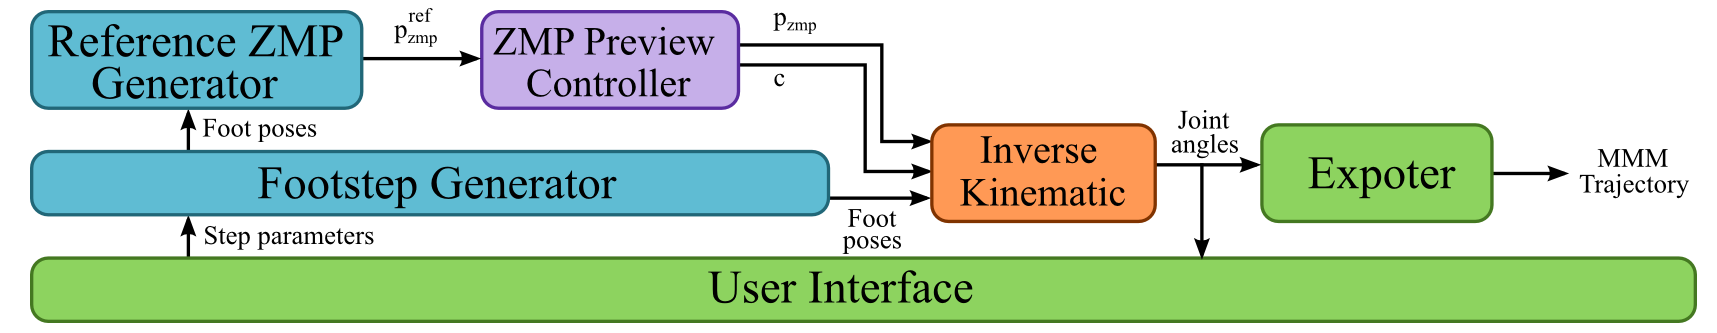
\includegraphics[width=\textwidth]{images/pattern_generator_architechture.png}
  \end{center}
\end{figure}

\end{frame}

\begin{frame}{Video of pattern based walking}

\begin{figure}
  \begin{center}
     \includemovie[poster]{6cm}{4cm}{../Videos/10_steps_unstabilized.mp4}
  \end{center}
\end{figure}

\end{frame}

\section{Walking Stabilization}\label{walking-stabilization}

\begin{frame}{Stabilizer}

\begin{itemize}
\itemsep1pt\parskip0pt\parsep0pt
\item
  \textbf{Problem:} Disturbances cause instabilities (even though the
  pattern is dynamically stable!)
\item
  \textbf{Solution:} Adapt pattern to disturbances \(\rightarrow\)
  stabilizer
\item
  \textbf{Implemented:} Stabilizer based on Kajita et al. 2010
  \cite{kajita2010biped}. Adapts frames in Cartesian space (no torque
  control needed).
\end{itemize}

\begin{figure}
  \begin{center}
     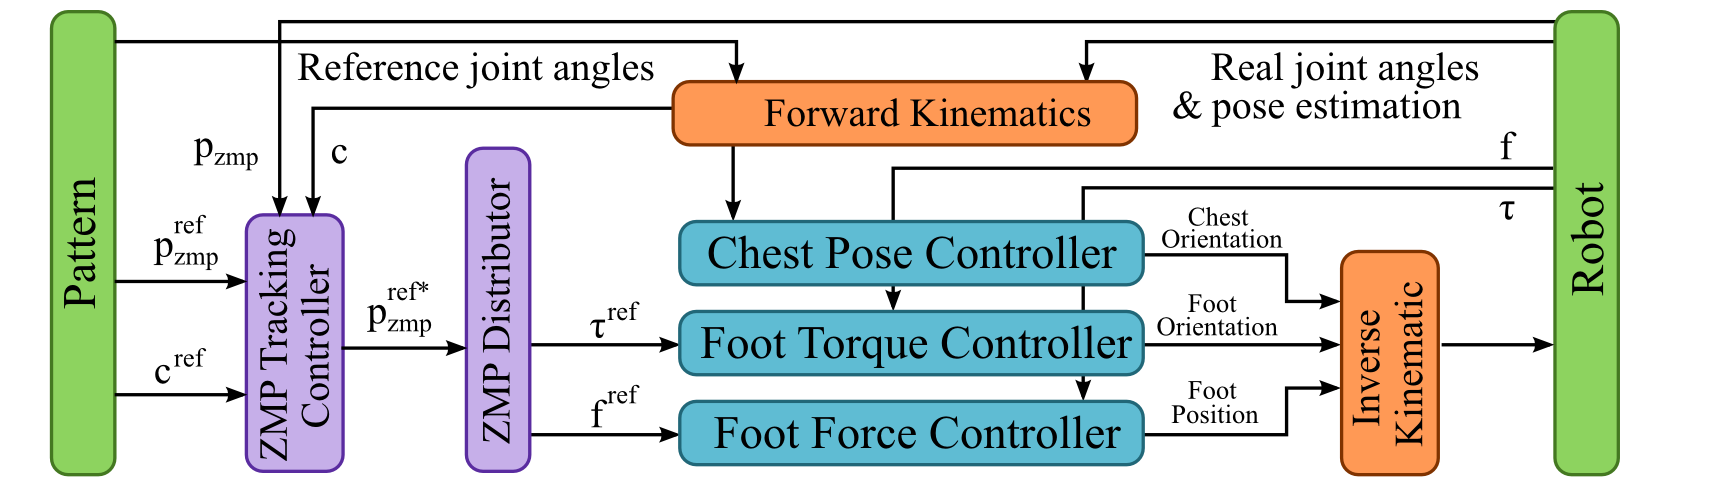
\includegraphics[width=\textwidth]{images/stabilizer_architechture.png}
  \end{center}
\end{figure}

\end{frame}

\begin{frame}{Ankle torques}

\textbf{Problem:} Needs accurately measured torques. Bullet does not
provide realistic torques.

\begin{figure}
  \begin{center}
     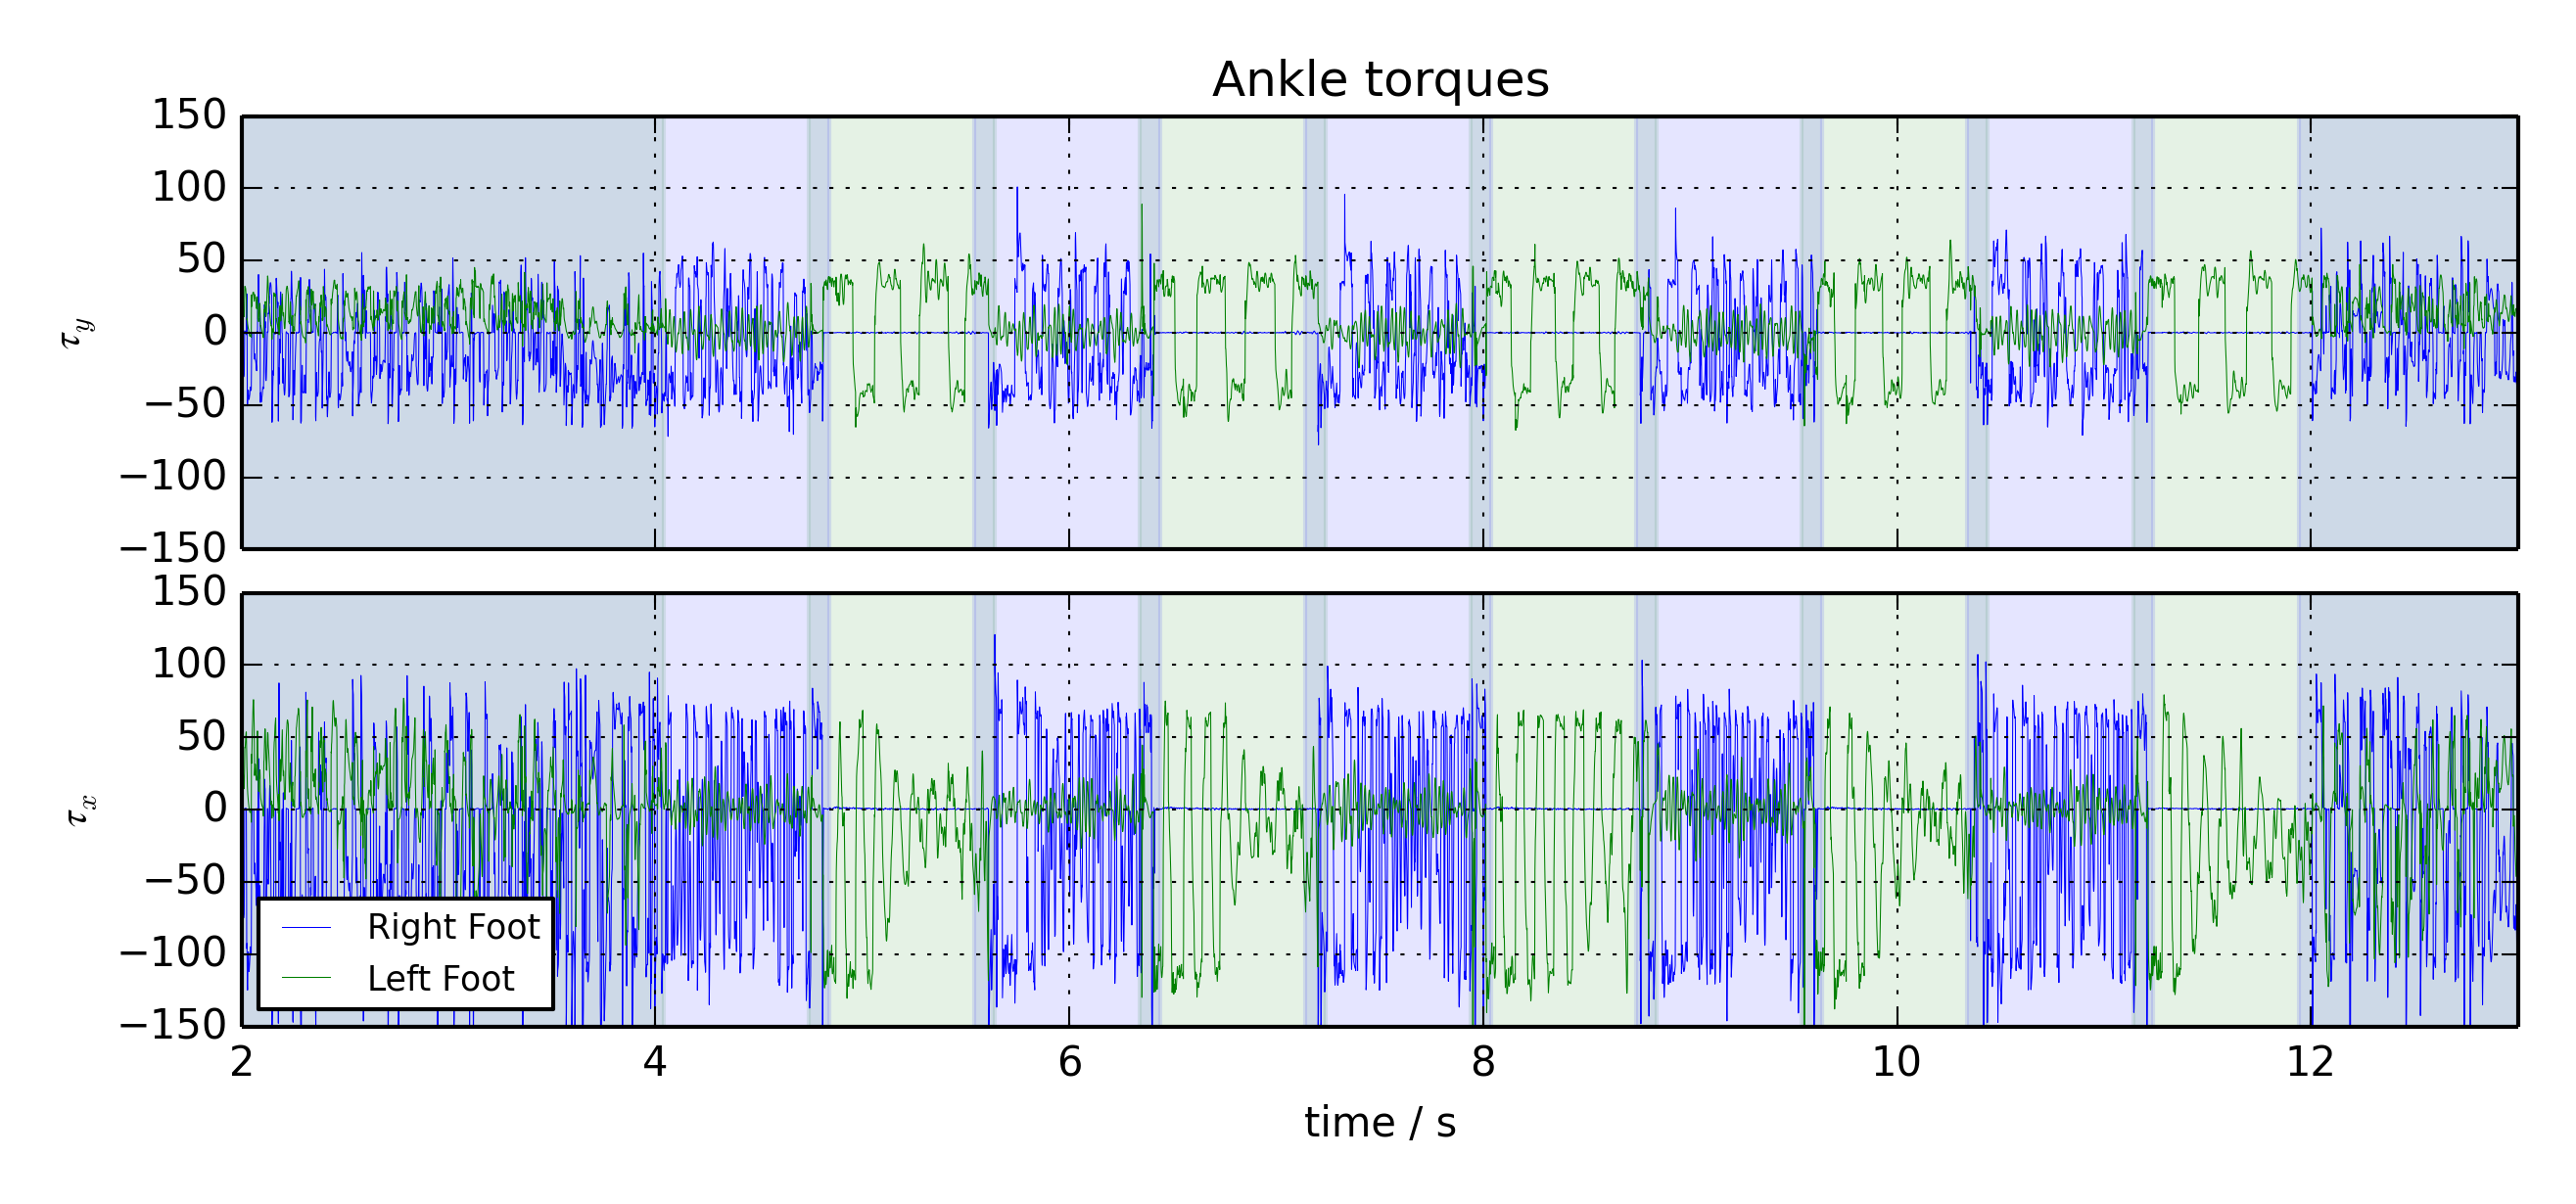
\includegraphics[width=\textwidth]{images/ankle_torques.png}
  \end{center}
\end{figure}

\end{frame}

\begin{frame}{Heuristic Stabilizer}

\begin{itemize}
\itemsep1pt\parskip0pt\parsep0pt
\item
  Works very similar to stabilizer proposed by Kajita
\item
  Instead of torque feedback, we use the pose of error of the frames
\item
  \textbf{Problem}: Accurately measuring pose error for each frame not
  possible in reality
\end{itemize}

\begin{figure}
  \begin{center}
     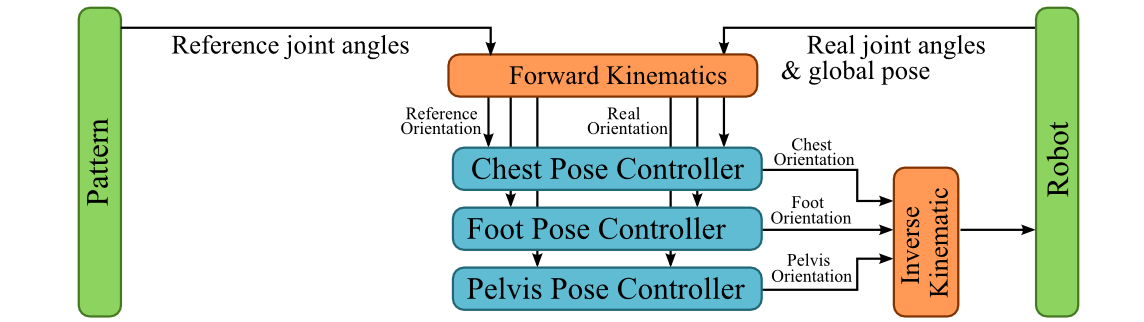
\includegraphics[width=\textwidth]{images/heuristic_architechture.png}
  \end{center}
\end{figure}

\end{frame}

\begin{frame}{Stabilized walking in a circle}

\begin{figure}
  \begin{center}
     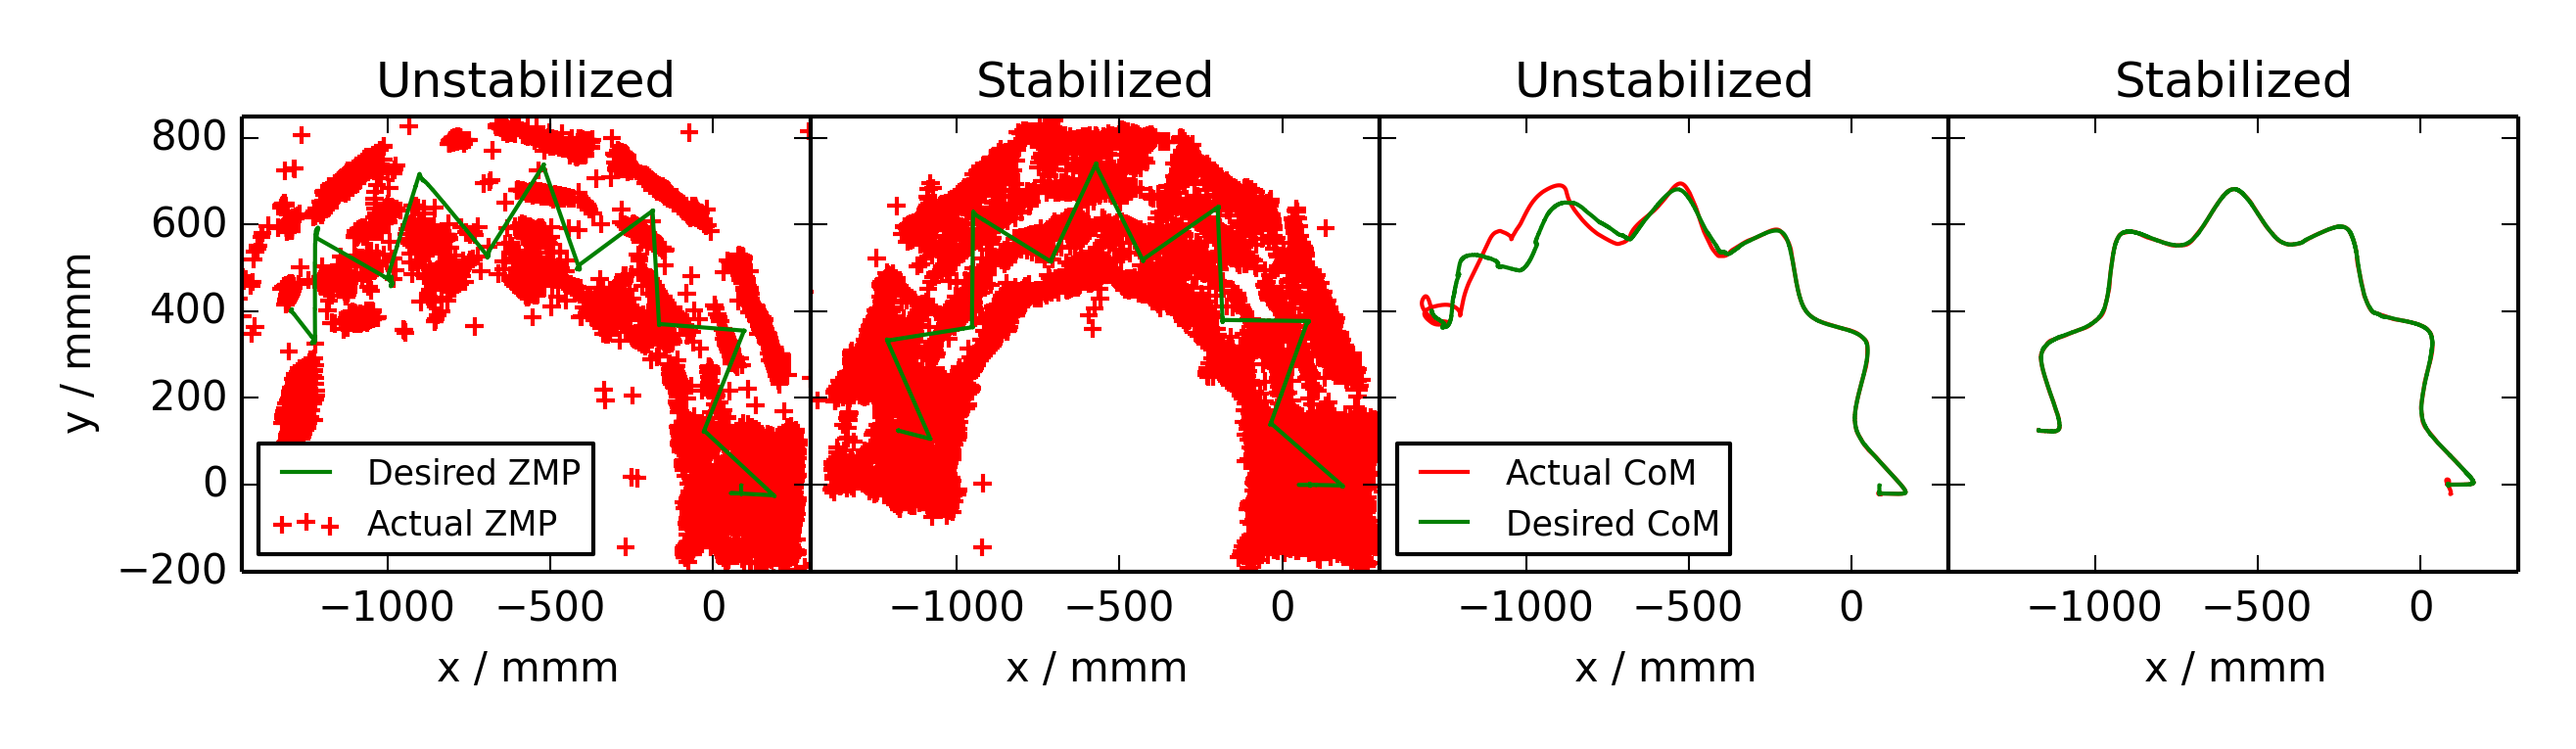
\includegraphics[width=\textwidth]{images/undisturbed_circle.png}
  \end{center}
\end{figure}

\begin{figure}
  \begin{center}
     \includemovie[poster]{3cm}{2cm}{../Videos/circle.mp4}
  \end{center}
  \caption{Walking in a half-circle.}
\end{figure}

\end{frame}

\begin{frame}{Walking with disturbances}

\begin{figure}
  \begin{center}
     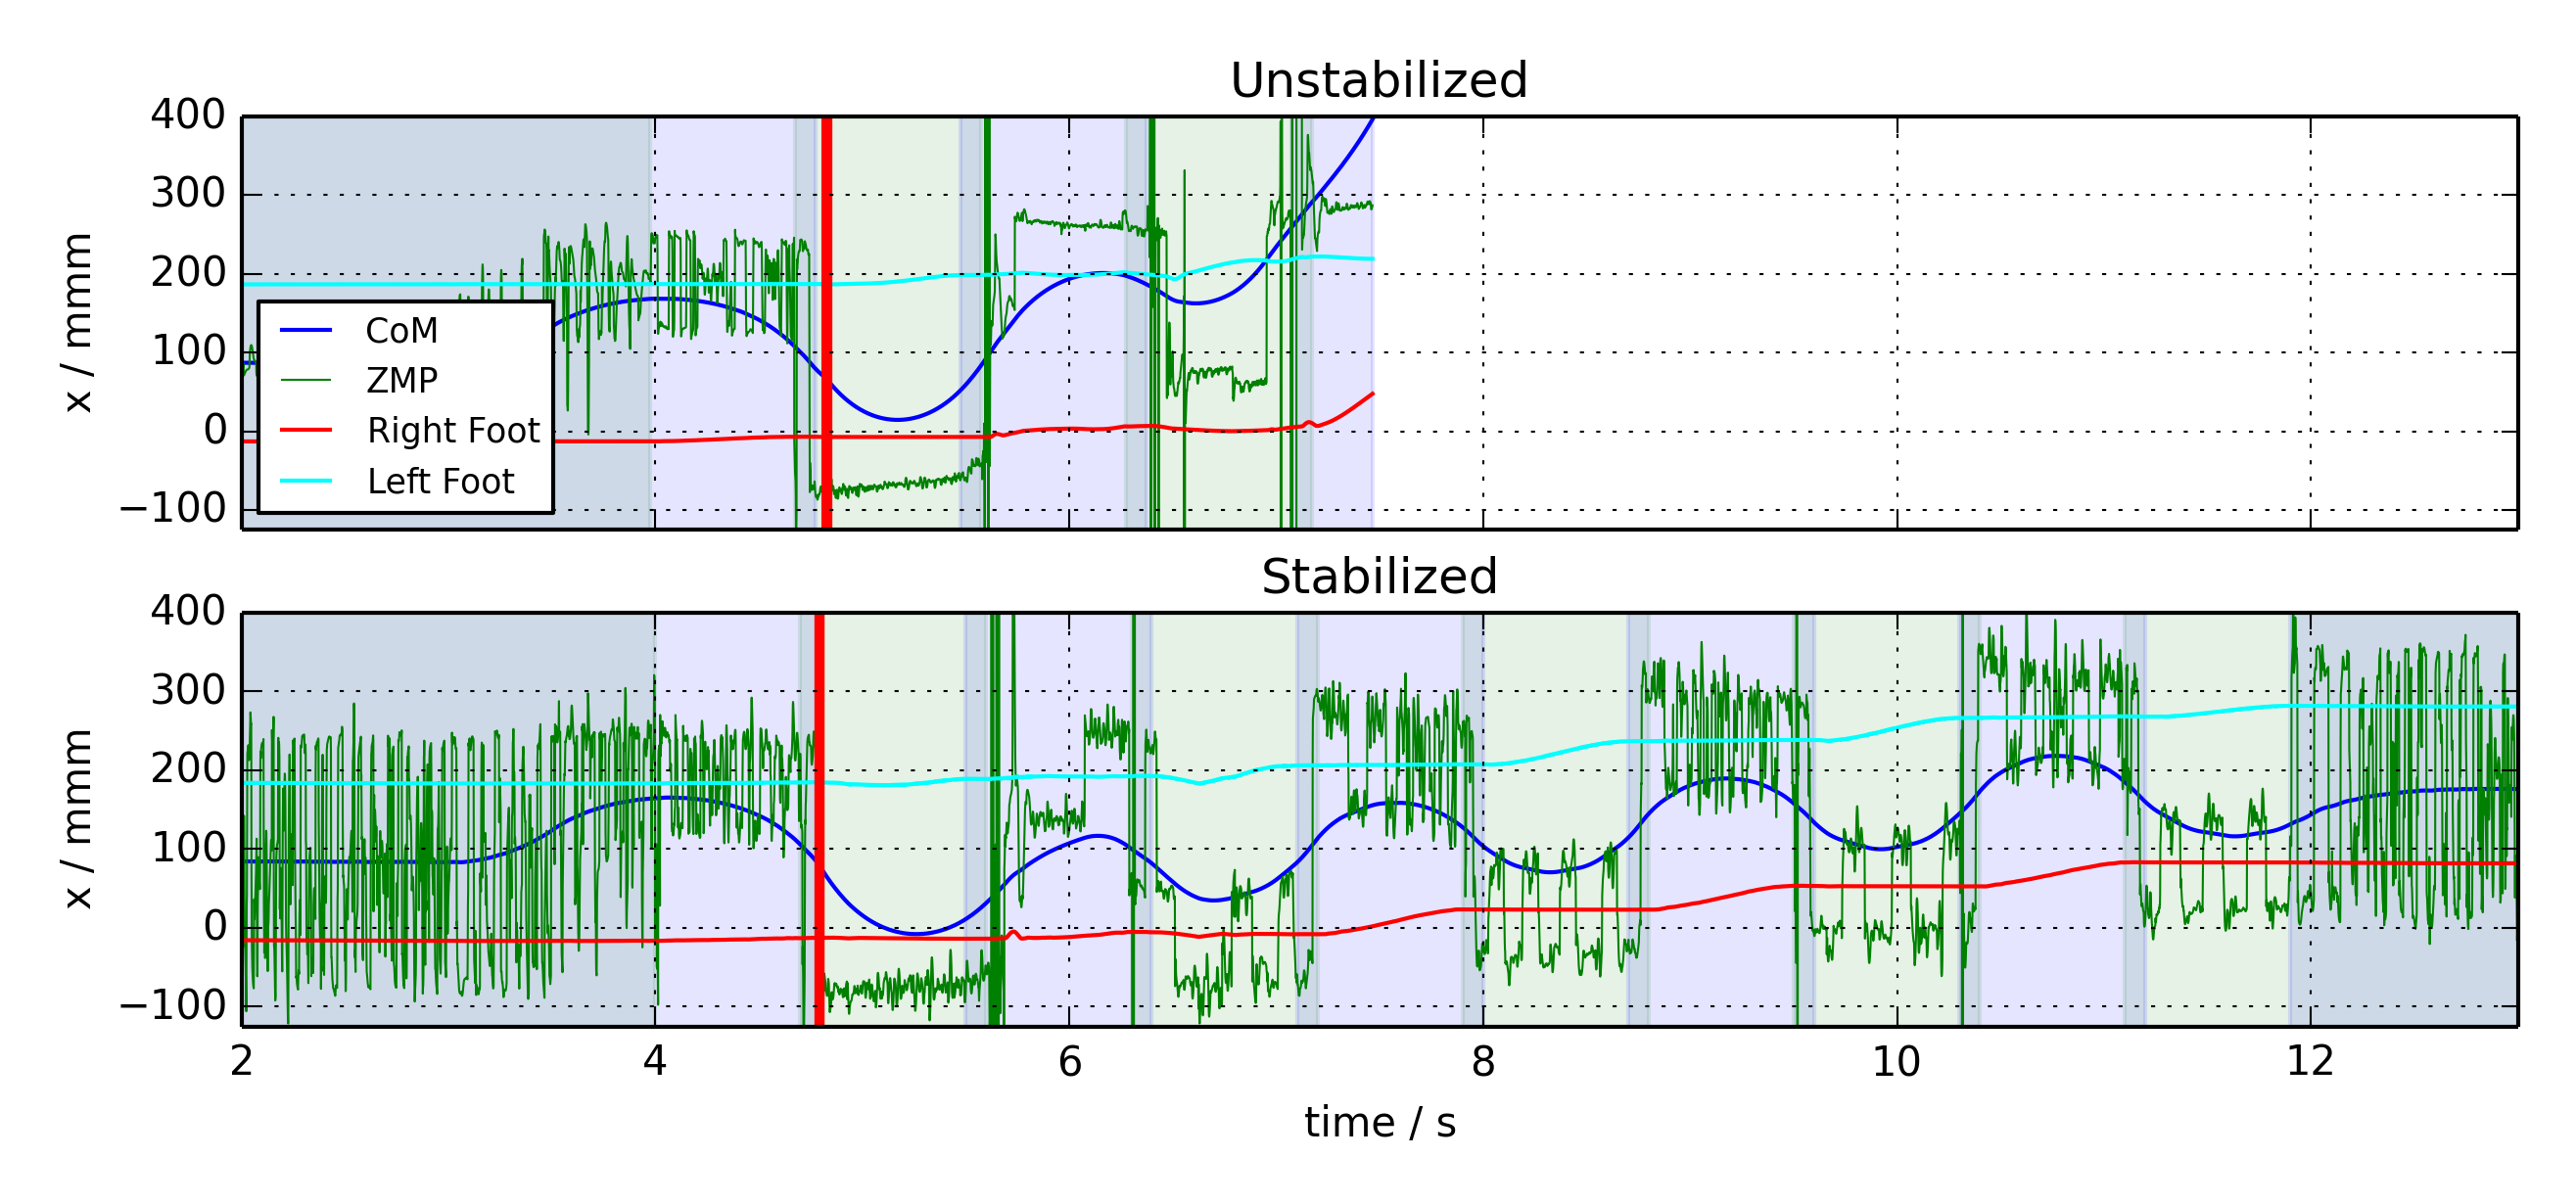
\includegraphics[width=\textwidth]{images/disturbed_front_straight_x.png}
  \end{center}
\end{figure}

\vspace{-2.5em}\begin{columns}
\begin{column}{5cm}
\begin{figure}
  \begin{center}
     \includemovie[poster]{5cm}{1cm}{../Videos/push_front_unstabilized.mp4}
  \end{center}
  \caption{Push without stabilization}
\end{figure}
\end{column}

\begin{column}{5cm}
\begin{figure}
  \begin{center}
     \includemovie[poster]{5cm}{1cm}{../Videos/push_front.mp4}
  \end{center}
  \caption{Push with stabilization.}
\end{figure}
\end{column}

\end{columns}

\end{frame}

\section{Push recovery}\label{push-recovery}

\begin{frame}{Push recovery based on Capture Point}

\begin{itemize}
\item
  The (immediate) Capture Point is defined as the point on the floor,
  where by placing the base of the pendulum there, the CoM would come to
  a rest. \cite{koolen2012capturability}
\item
  \textbf{Problem:} The base needs to be moved instantaneously to the
  Capture Point, but foot would at least need \(t_{min}\) seconds.
\item
  \textbf{Solution:} Predict the future position of the immediate
  Capture Point in \(t_{min}\)
\end{itemize}

\begin{figure}
  \begin{center}
     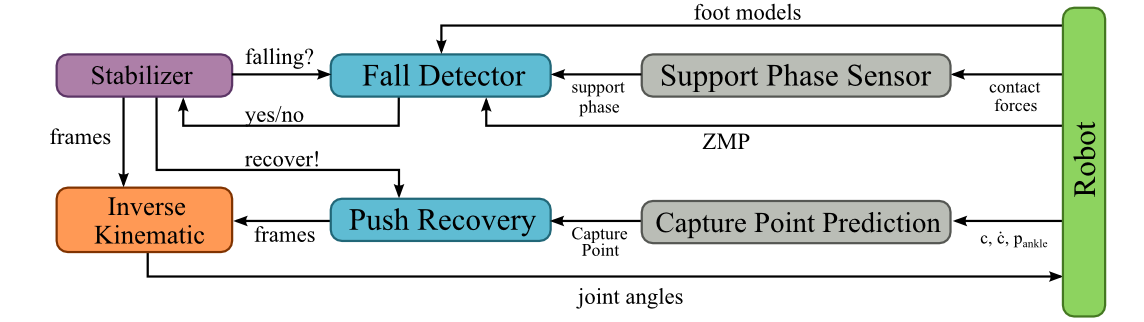
\includegraphics[width=\textwidth]{images/recovery_architechture.png}
  \end{center}
\end{figure}

\end{frame}

\begin{frame}{Capture Point Video}

\begin{figure}
  \begin{center}
     \includemovie[poster]{5cm}{5cm}{../Videos/recovery.mp4}
  \end{center}
  \caption{Push recovery, standing on left leg.}
\end{figure}

\end{frame}

\section{Conclusion \& Future Work}\label{conclusion-future-work}

\begin{frame}{Implementation}

\begin{itemize}
\item
  All algorithms implemented independent of the physical simulation
  (\texttt{libBipedal}): \texttt{https://github.com/TheMarex/libbipedal}
\item
  Simulator using Simox with SimDynamics:
  \texttt{https://i61wiki.itec.uka.de/git/simdynamicsviewer.git}
\item
  All C++11, needs Simox, MMMCore and Bullet 2.82 with double support
\end{itemize}

\begin{figure}
  \begin{center}
     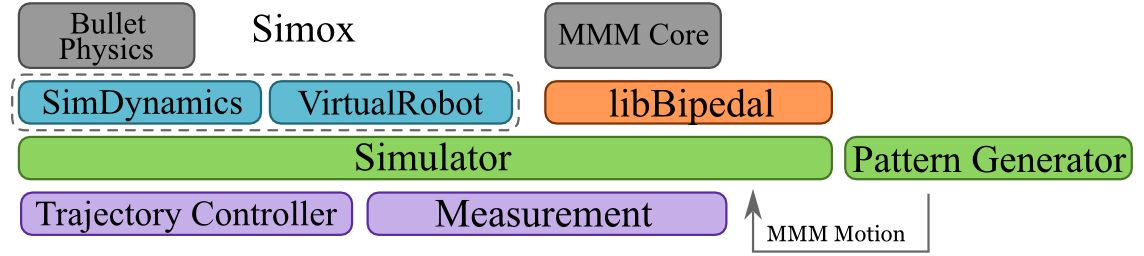
\includegraphics[width=\textwidth]{images/architechture.png}
  \end{center}
\end{figure}

\end{frame}

\begin{frame}{Conclusion}

\begin{itemize}
\itemsep1pt\parskip0pt\parsep0pt
\item
  Implemented a \textbf{dynamic simulator} that can test MMM
  trajectories
\item
  \textbf{Verified} walking patterns in dynamic simulation
\item
  Implemented multiple \textbf{stabilizers} and tested in simulation
\item
  Implemented simple \textbf{push recovery} mechanism based on the
  Capture Point
\end{itemize}

\end{frame}

\begin{frame}{Future Work}

\begin{itemize}
\item
  Implement different pattern generation schemes (simple 3D-LIPM based,
  CP based)
\item
  Make walking more natural: Use toe joint. \(\rightarrow\) Kajita et
  al. \cite{kajita2012evaluation} proposed extension of the methodes
  implemented here to include a toe support phase
\item
  Better push recovery: General case, use extended LIP models proposed
  by Pratt
\end{itemize}

\end{frame}
